\section{Performance Evaluation}\label{sec:evaluation}

When operating a service, the overall performance objective is to provide acceptable service latency at minimal cost. The cost can be lowered by running fewer servers - but this increases the latency because requests spend more time waiting for contended resources (such as network, storage, CPU, threads, locks, and so on). This tradeoff is an essential challenge for developers writing an elastic service application. 

To clarify the value that our automatic change propagation provides to service architects, we now quantify both (a) its latency overhead and (b) its resource consumption, by comparing them to alternative solutions, including periodic polling (\S\ref{sec:polling}) and explicit change propagation at the application level (\S\ref{sec:observers}). To this end, we designed two series of experiments that measure low-load latency (\S\ref{sec:latency}), and variable-load throughput (\S\ref{sec:throughput}).

\mypar{Application Model}  
We model the application using  \emph{item} grains that are observed by \emph{view} grains. Each view depends on a fixed number of items, selected at random at the beginning of the test. Views are updated when items change, in a manner that depends on the chosen propagation solution, one of \emph{polling} (\S\ref{sec:polling}), \emph{explicit propagation} (\S\ref{sec:observers}), or \emph{automatic propagation} (\S\ref{sec:reactive}). Moreover, we vary the number of items and views to simulate different workloads (Table~\ref{tab:param}).  For example, a high \emph{fan-out} (= average number of views that depend on an item) means that whenever an item is mutated, many views need to be updated. 

The items and views run on five Orleans silos deployed as a Windows Azure cloud service. The robots run on 10 load generator servers. All processors have 8 cores, 14GB of RAM, and run at 1.6 GHz. To account for unexpected variations, we made sure to run each experiment series on at least 2 different datacenters, on at least 3 different days, and running the experiments in different order. Between runs, absolute numbers can vary up to 10\%, but the relative performance of the various solutions were stable. Note that we achieved this only after investing substantial work into our experimentation framework. 

Note that by design, this is a microbenchmark that isolates the mechanism we want to measure (change propagation) and removes all other aspects. If deployed as part of a complete service, including item persistence, the performance differences between the various solutions are likely to be less pronounced.
 
\begin{table}
\begin{tabularx}{.99\columnwidth}{@{}Xrrrr@{}} \toprule
Name		& \#items 	& \#views & \#deps. & max robots\\ \midrule
low-load	&  600        	& 20       & 4 & n/a \\
fanout-1	& 20,000	& 20,000 & 1& 2,000 \\
fanout-20	& 10,000	& 20,000 & 10 & 2,000\\
fanout-200 & 1,000	& 20,000 & 10& 1,000\\  
\end{tabularx}
\caption{Parameter combinations we used.}\label{tab:param}
\end{table}


\subsection{Latency}\label{sec:latency}

Our latency experiments use the low-load parameters (Table~\ref{tab:param}) to eliminate delays caused by queueing and contention. We measure two types, called \emph{query latency} and \emph{propagation latency}. Latencies are measured 4000 times each (200 times per view, separated by 500ms). We describe the results using the median and lower and upper quartiles.\footnote{Average and standard deviation are unsuitable statistics because of the long tail of the distribution.}

\subsubsection{Query Latency}

\begin{figure}
\begin{lstlisting}
grain View
{
	state Deps: Item[numdeps]; 
	op Query(sequential: bool) : int[]
	{	
		var result = new int[numdeps];
		if (sequential) {
			for (0 <= i < numdeps)
				result[i] = Deps[i].GetValue();
		} else {
			parallel for (0 <= i < numdeps)
				result[i] = Deps[i].GetValue();
		}
		return result;
	}
	op OneTimeReactiveQuery(sequential: bool) : int[]
	{
	 	var rc = CreateReactiveComputation(
	 										() => Query(sequential));
		var result = await rc.GetResultTracker.NextResult();
		rc.Dispose();
		return result;
	}
}
\end{lstlisting}
\caption{Queries expressing how views depend on items.}\label{fig:queries}
\end{figure}

\begin{figure}
\centering
\begin{tabular}{@{}c@{}}
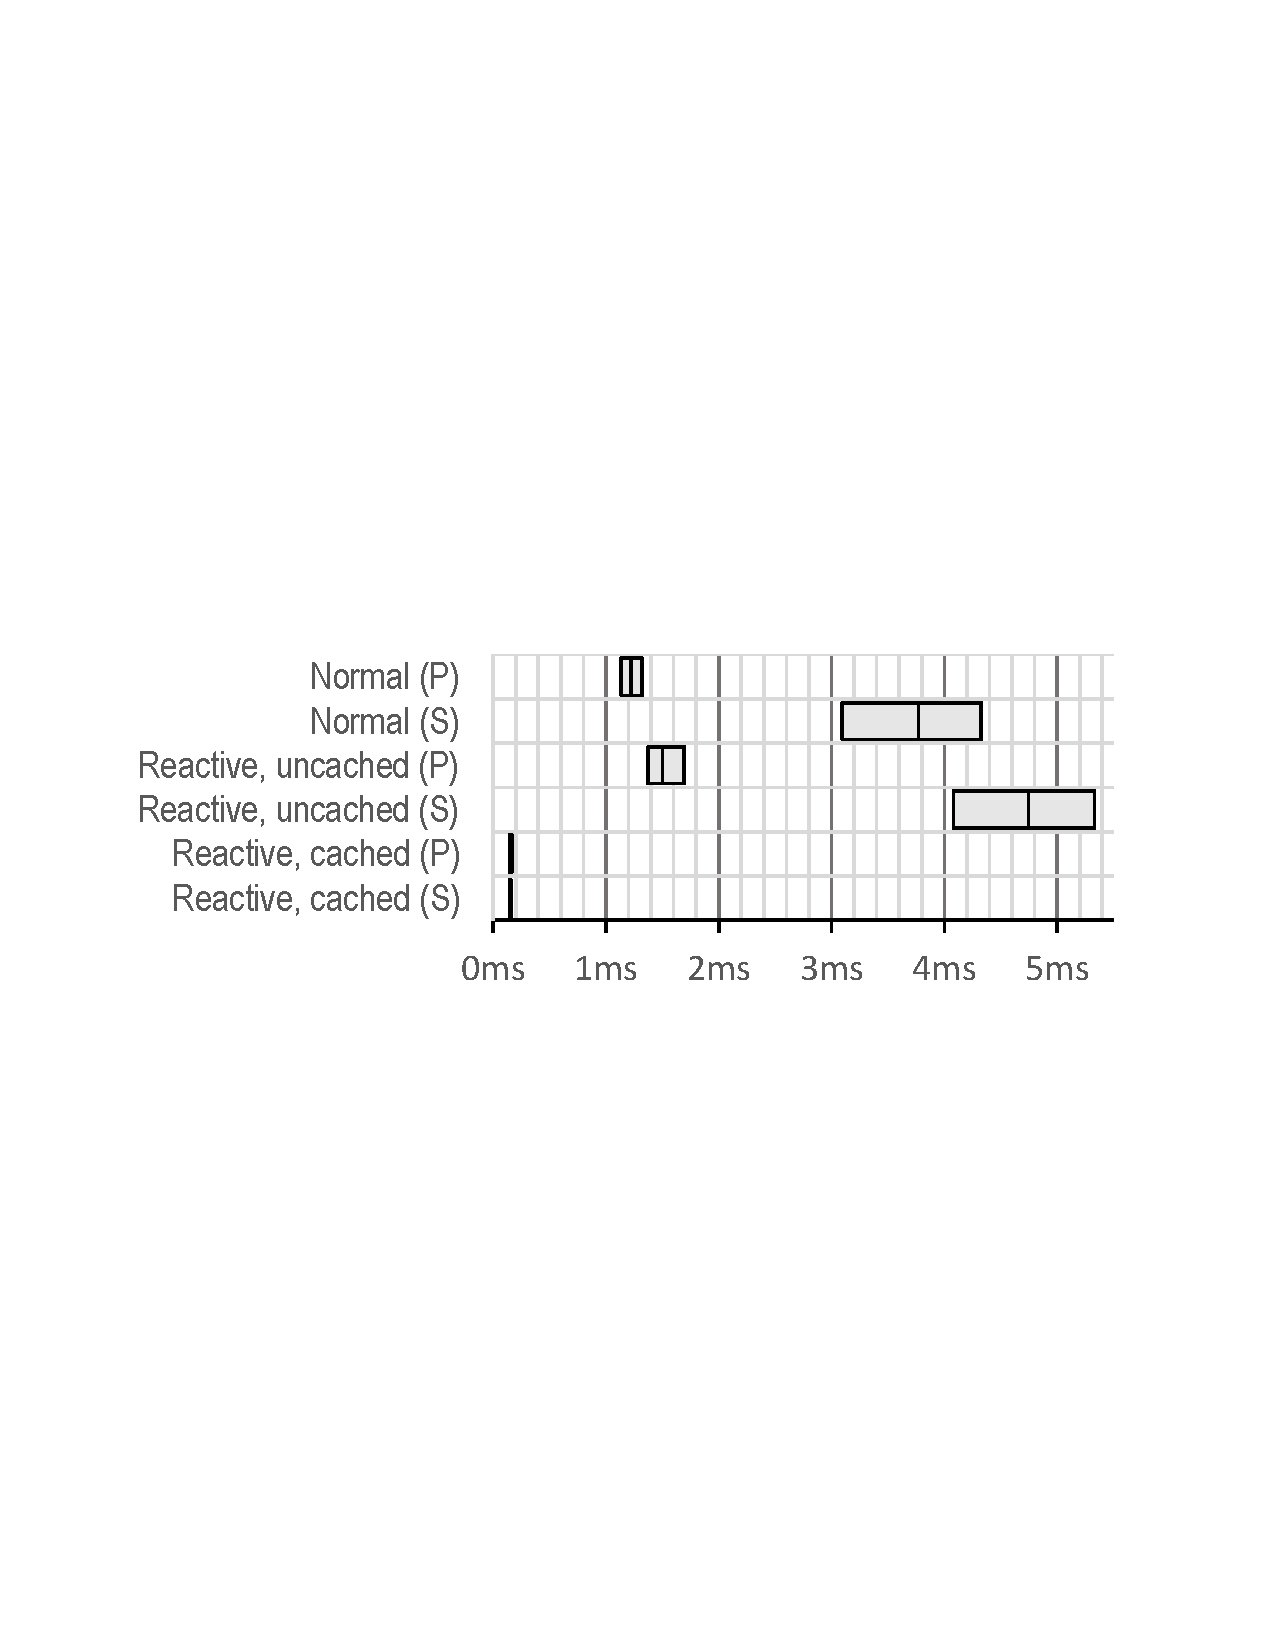
\includegraphics[width=\columnwidth, viewport=67 322 534 477]{figs/query-latencies}\\[.2in]
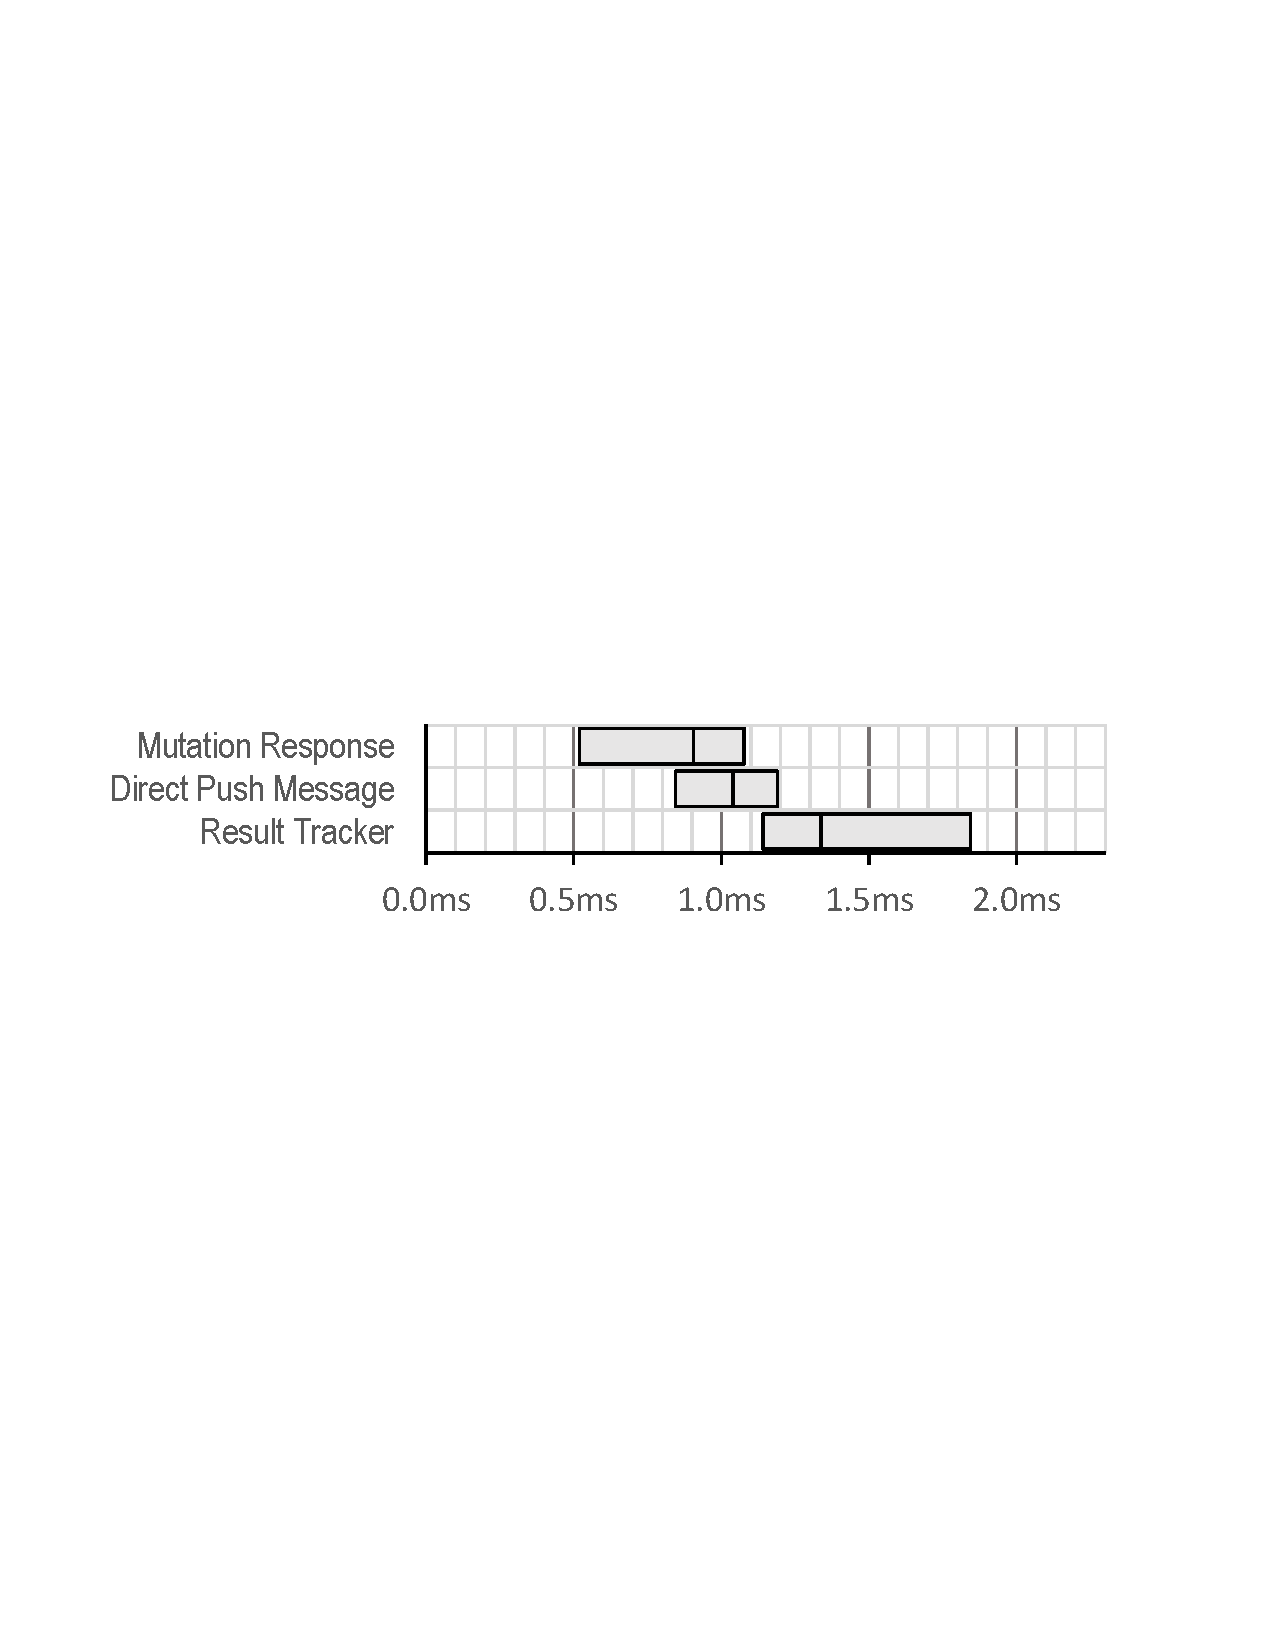
\includegraphics[width=\columnwidth, viewport=54 354 530 444]{figs/push-latencies}\\[.2in]
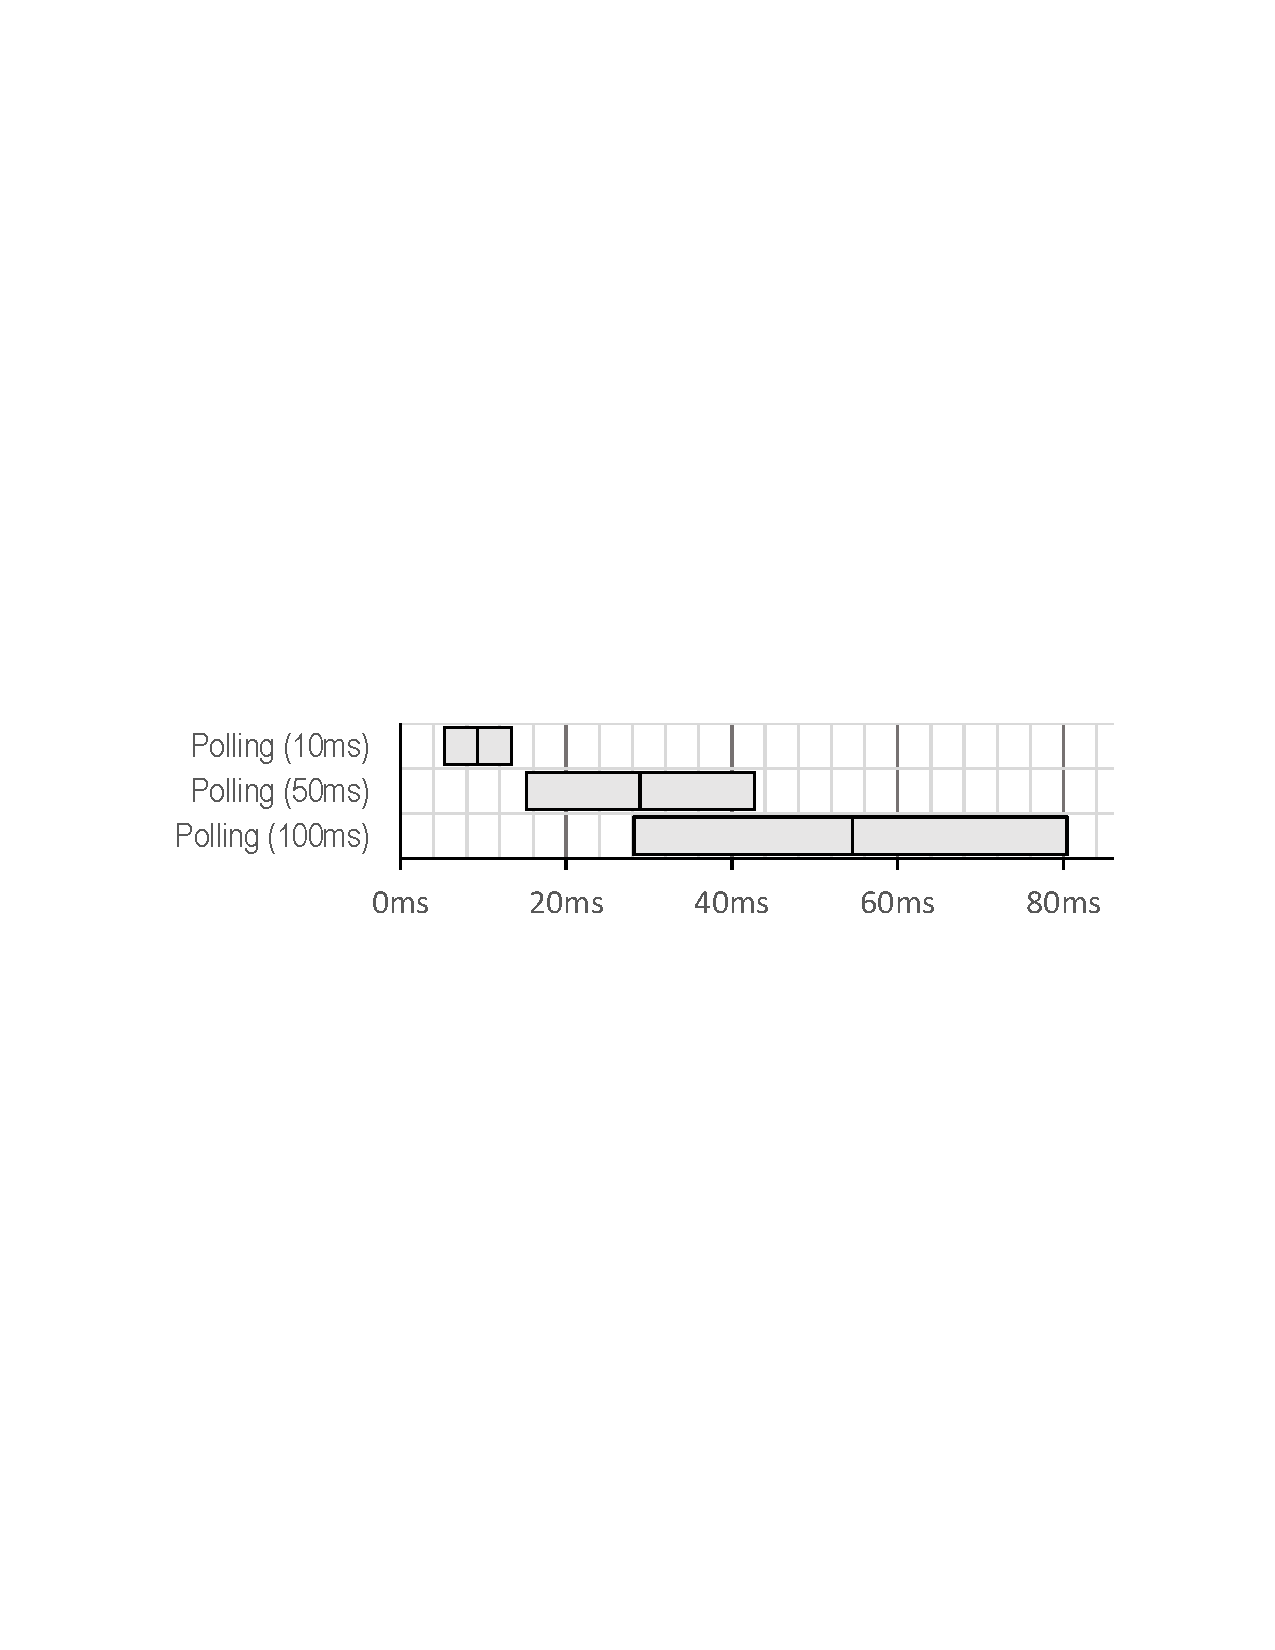
\includegraphics[width=\columnwidth, viewport=85 354 534 444]{figs/polling-latencies}\\
\end{tabular}
\caption{Measured latencies under low load, in milliseconds. The line in the middle of each box is the median, and the left and right edge are the first and third quartile. \textbf{(top)} Latencies for parallel and sequential queries; \textbf{(middle)} latencies for mutation response, application-level propagation using direct messages, and automatic propagation using result trackers; \textbf{(bottom)} propagation latencies for the polling solution at various frequencies.}\label{fig:querylatencies}
\end{figure}

For measuring query latency, we execute a query on a view that calls each of four items (either sequentially or in parallel) to collect some value and returns the values in an array (Fig.~\ref{fig:queries}). We now compare the latency when executed normally (\lstinline|Query|) to the latency when executed as a reactive computation (\lstinline|OneTimeReactiveQuery|). The normal latency for the sequential and parallel versions are shown in the first two rows of Fig.~\ref{fig:querylatencies} (top). The median latency is about 1.2ms for the parallel query and 3.8ms for the sequential query. This is consistent with the round-trip time of a typical grain call taking a bit less than 1ms. For the reactive queries, we distinguish two cases. If  the relevant summaries are not already cached on the silo, the query takes about 25\% longer than normal (rows 2,3). This overhead is caused by the installation and removal of the summary caches, and by scheduling overhead of our reactive caching implementation. However, if summaries for the items are already cached on the silo (for example, if another view is tracking the same items), the latency of \lstinline|OneTimeReactiveQuery| is less than 200$\mu$s (rows 4,5) because remote calls can be completely avoided. 

\paragraph{Conclusions.} The results demonstrate that (1) the latency overhead of constructing the dependency graph is modest, and (2)  the caching effect alone can improve latency, even if not using the reactive features.

\subsubsection{Propagation Latency}

For measuring propagation latency, a view sends an update message to an item it depends on, and measures how much time elapses (a) until it receives the mutation response, and (b) until it receives the change propagation. 

First, we measured the speed of explicit propagation, where each item sends a notification message to all dependent views when mutated. This establishes a lower bound on propagation speed in the Orleans framework. The results show that the propagation message arrives right after the mutation completes: close to 1ms after calling the mutation operation (rows 2,3 of Fig.~\ref{fig:querylatencies} (middle)). This is consistent with the underlying system sending the mutation response message and the propagation message at about the same time. 

Second, we measured the speed of automatic propagation provided by our reactive caching algorithm. In that case, the propagation takes about 300$\mu$s longer (row 3), due to the scheduling overhead of our implementation.

Finally, we looked at the propagation speed of a polling-based solution. Fig.~\ref{fig:querylatencies} (bottom) shows the measured latencies, using a sequential query and various polling intervals. As expected, we see a median propagation time in the neighborhood of half of the polling interval plus the query latency, and a wide inter-quartile distance. However, polling every 100ms is usually not advisable (we show impact of polling on throughput in \S\ref{sec:throughput}). Reasonable polling intervals are more typically between 1 and 30 seconds, with a median propagation speed that is easily three orders of magnitude worse than for explicit or automatic change propagation.  

\paragraph{Conclusions.} The results show that our automatic propagation performs much better than a polling solution, while having the same simple programming model; and is not much slower than explicit change propagation.


\subsection{Throughput}\label{sec:throughput}

For the throughput experiments, we generate external load as shown in Fig.~\ref{fig:tp-setup}. The load generator contains up to 2000 robots; each runs a continuous loop that sends requests to the service, either to read a view, or to update an item. The percentage of updates in the mix is configurable. 

\begin{figure}
\centering
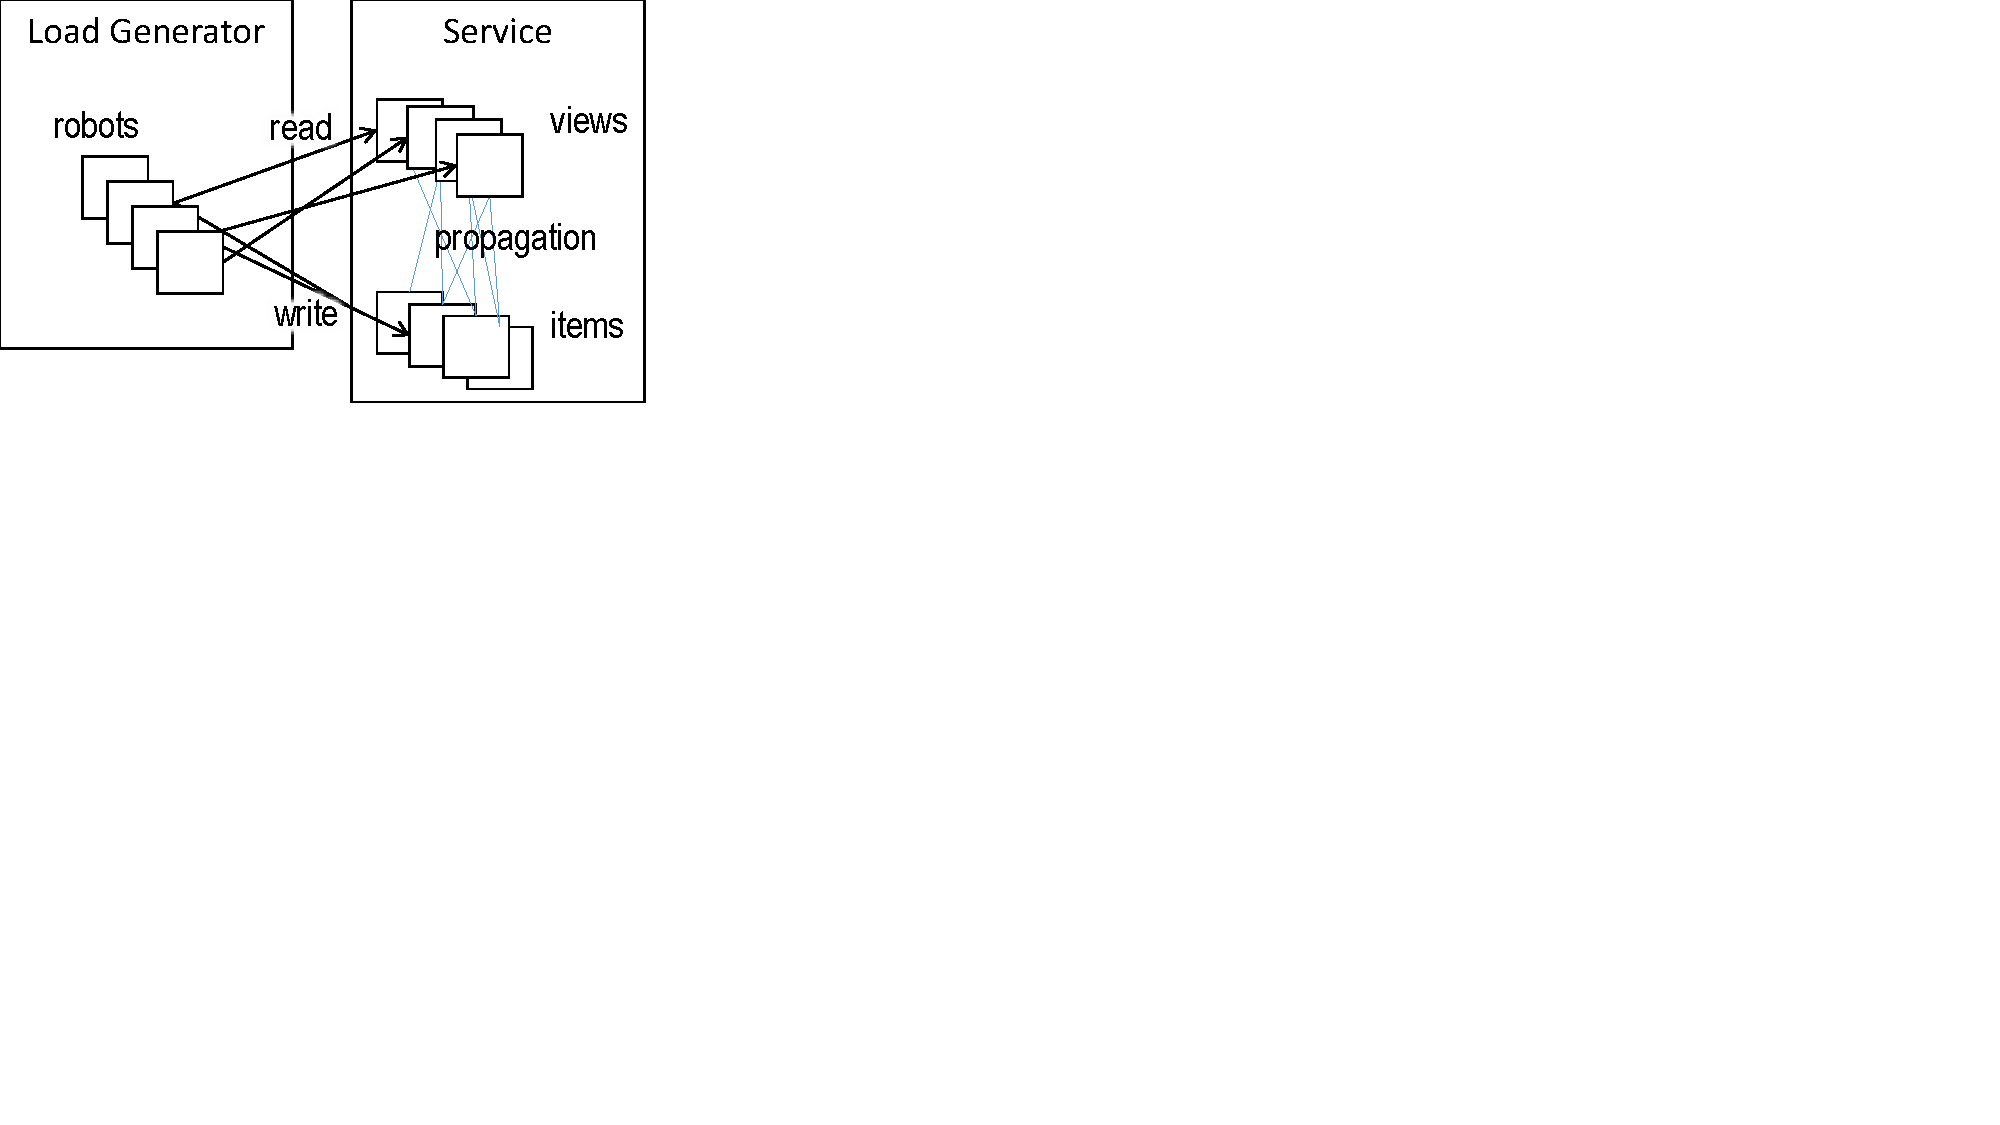
\includegraphics[scale=.5, viewport=0 346 309 540]{figs/tp-setup} 
\caption{Experimental setup for throughput experiments.}\label{fig:tp-setup}
\end{figure}

\begin{figure}
\noindent
\centering
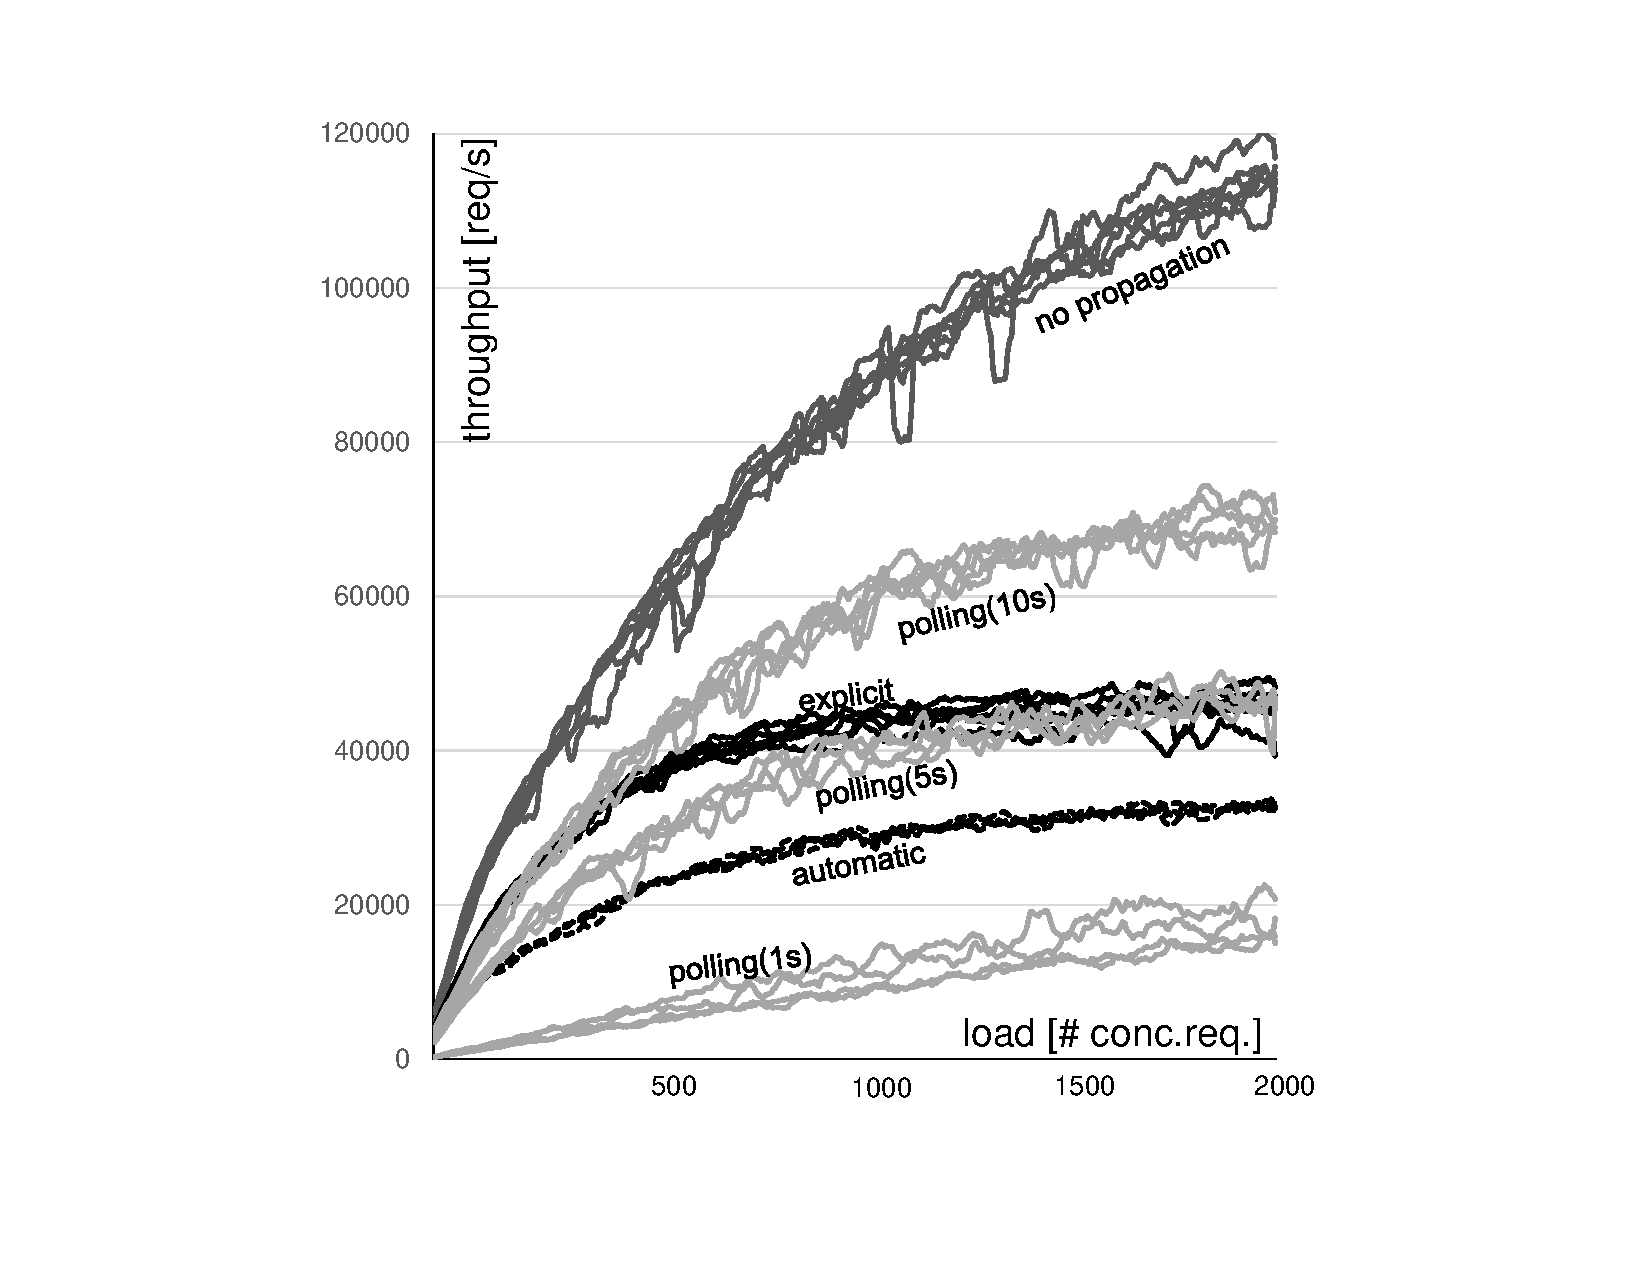
\includegraphics[width=\columnwidth, viewport=154 86 630 553]{figs/tp-curves} 
\caption{Throughput response of different propagation mechanisms, for fanout-20 with 10\% updates.}\label{fig:tp-curves}
\end{figure}
\begin{figure*}
\noindent
\centering
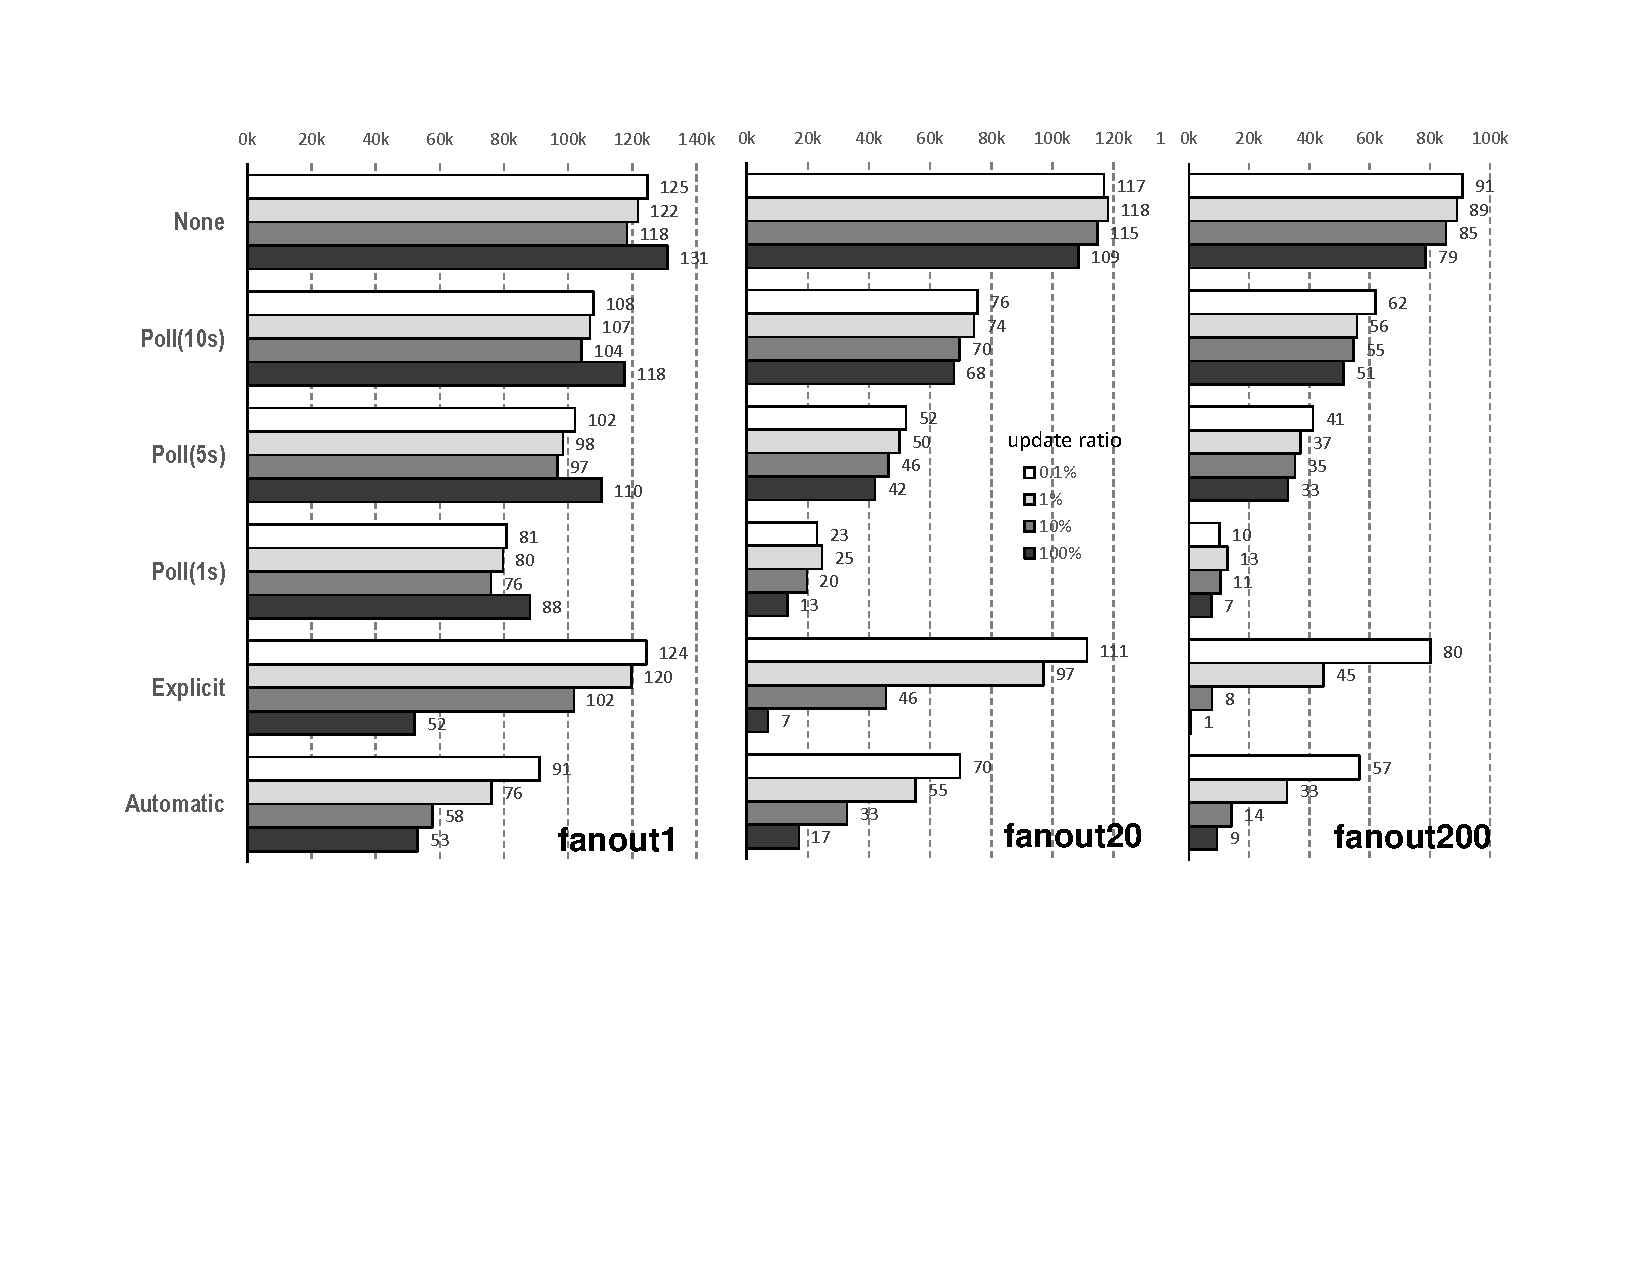
\includegraphics[width=\textwidth, viewport=58 195 726 550]{figs/tp-all} 
\caption{Measured throughput (in thousands of requests per second) for varying configurations (Table~\ref{tab:param}), propagation mechanisms, and percentage of updates.}\label{fig:tp-all}
\end{figure*}

Each experiment gradually increases the robots and measures the throughput over time. The result is a curve that shows how throughput (number of requests handled per second) responds to load (number of requests concurrently in flight). For example, for the \lstinline|fanout20| configuration and a request mix containing 10\% updates, we obtained the curves shown in Fig.~\ref{fig:tp-curves}; each line corresponds to one experiment, and each bundle of similar lines corresponds to several experiments using the same propagation mechanism. 

The best possible throughput is achieved when change propagation is turned off entirely - because all resources are used for handling requests. Here, we reach close to 120k requests per second. But as soon as we use change propagation mechanism, the throughput is lower, because resources diverted to the propagation mechanism: explicit propagation (dotted lines) reaches about 45k, automatic  propagation reaches about 35k. For 10s-polling, the throughput reaches about 70k (better than automatic or manual propagation), but for 1s-polling, it reaches only about 20k (worse than automatic or manual propagation). 

To compare the solutions across different configurations and update ratios, we ran this type of experiment for all combinations, but extended to run fixed load (the maximum number of robots as in Table~\ref{tab:param}) for a while at the end, to measure average  peak throughput for that load. The results are shown in Fig.~\ref{fig:tp-all}. Each column corresponds to a configuration in Table~\ref{tab:param}); each row corresponds to a choice of propagation mechanism; and each bar color corresponds to update percentage. For example, the dark gray bars (10\% updates) in the middle column (fanout20) correspond to the peak throughput in Fig.~\ref{fig:tp-curves}

\mypar{Baseline} With update propagation turned off (top row, labeled \emph{None}), all requests are simple operations on a single grain. We reach a throughput in the neighborhood of  120k for the fanout1 and fanout20 configurations (under a load of 2000 concurrent requests), and near 90k for the fanout200 configuration (under load of 1000 concurrent requests). Though throughput is largely consistent, the numbers show some unexpected variation: throughput degrades somewhat with higher update percentages, and jumps up for the specific combination of fanout1 and 100\% updates). We suspect they are caused by load balancing differences within the Orleans runtime regarding items, views, and requests.

\mypar{Polling} The extra work incurred by polling is (a) inversely proportional to the polling interval, and (b) proportional to the number of items a view depends on. The reduction in throughput (relative to the baseline) is thus modest for views that depend on only 1 item (left column), especially for large polling intervals, but if the view depends on 10 items (middle and right column), the throughput reduction is significant.

\mypar{Explicit Propagation} The extra work incurred by explicit propagation is proportional to both the percentage of updates and the fan-out. The results confirm this: (1) we see o.k. throughput results for update percentages up to 1\%, and (2) we see terribly low throughput for the combination of high fanout and high update percentage, as low as 1k (lowest of all) for fanout200 and 100\% updates.

\mypar{Automatic Propagation} There are two main differences between the work required for automatic and explicit propagation: (1) automatic propagation incurs a bit more work due to scheduling indirection, re-execution of summaries, and management of reactive caches;  and (2) automatic propagation can adapt to back-pressure and reduce the number of updates sent.  We can observe these effects: throughput for automatic propagation is generally lower than for explicit propagation, except for high update rates and/or fanout where explicit propagation suffers more. 
 
\mypar{Conclusions} The results show that automatic propagation is generally competitive with explicit propagation. It is even better in cases where there are many updates to be propagated, thanks to its batching optimization. Polling remains an acceptable solution for applications that do not require quick propagation time; it can be tuned to reliably consume little resources, even under high update rates.

 
 


